\documentclass[api,pof,pre,12pt,a4paper]{revtex4-1}     
\usepackage{bm}
\usepackage{natbib}
\usepackage{url}
\usepackage[intlimits]{amsmath}
\usepackage{graphicx}
\usepackage{fancyhdr}
\usepackage{amsfonts}
\usepackage{amssymb}
%\usepackage{pstricks}
%\usepackage{pst-coil}
%\usepackage{pst-plot}
\usepackage{hyperref}
\usepackage{float}
\usepackage{subfig}


\newtheorem{theorem}{Theorem}
\newtheorem{prob}{Problem}
\newenvironment{problem}[1]{\begin{prob} {\rm #1} \end{prob}}

%Nadir's Shortcuts
\newcommand{\beqn}{\begin{equation}}
\newcommand{\eeqn}{\end{equation}}
\newcommand{\beqa}{\begin{eqnarray}}
\newcommand{\eeqa}{\end{eqnarray}}
\newcommand{\beqanonum}{\begin{eqnarray*}}
\newcommand{\eeqanonum}{\end{eqnarray*}}
\newcommand{\beqnonum}{\begin{equation*}}
\newcommand{\eeqnonum}{\end{equation*}}
\newcommand{\jump}{\vspace{0.5cm}}
\newcommand{\bbf}{\begin{bf}}
\newcommand{\ebf}{\end{bf}}
%\newcommand{\eqnref}[1]{(\ref{#1})}
\newcommand{\defn}[1]{\begin{bf}\emph{#1}\end{bf}}
\newcommand{\reals}{\ensuremath{\mathbb{R}}}
\newcommand{\complex}{\ensuremath{\mathbb{C}}}
\newcommand{\integers}{\ensuremath{\mathbb{Z}}}
\newcommand{\half}{\ensuremath{\frac{1}{2}}}
\newcommand{\n}{\nonumber}
\renewcommand{\d}{\mathrm{d}}
\newcommand{\del}{\partial}
\newcommand{\dd}{\ensuremath{\, \mathrm{d}}}
\newcommand{\nint}[4]{\int_{#3}^{#4} {#1}\, \mathrm{d}{#2}}
\newcommand{\der}[2]{\frac{\d {#1}}{\d {#2}}}
\newcommand{\parder}[2]{\frac{\del {#1}}{\del {#2}}}
\newcommand{\funder}[2]{\frac{\delta {#1}}{\delta {#2}}}
\newcommand{\Lag}{\mathcal{L}}

\oddsidemargin  0.0in
\evensidemargin 0.0in
\textwidth      6.5in
\headheight     15pt
\topmargin      0.0in
\textheight=8.0in
%\setlength{\parindent}{0in}

\lhead{Wavelength competition in modified SH}
\chead{}
\rhead{Gandhi et al.}
%\lfoot{}
%\cfoot{}
%\rfoot{}


%Figures
\newcommand{\FIGmarginalstability}{
\begin{figure}[t]\center
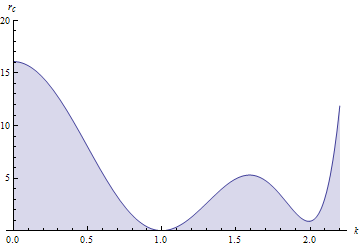
\includegraphics[width=60mm]{MarginalStability.png}
\caption{\label{fig:marginalstability} Linear stability of the modified Swift-Hohenberg equation with $q=2$ and $\delta=.1$.  The shaded region indicates linearly stable parameter regimes of the homogeneous solution with a forcing $r$ for a given wavenumber $k$.}
\end{figure}
}
\newcommand{\FIGbifurcationdiagramA}{
\begin{figure}[t]\center
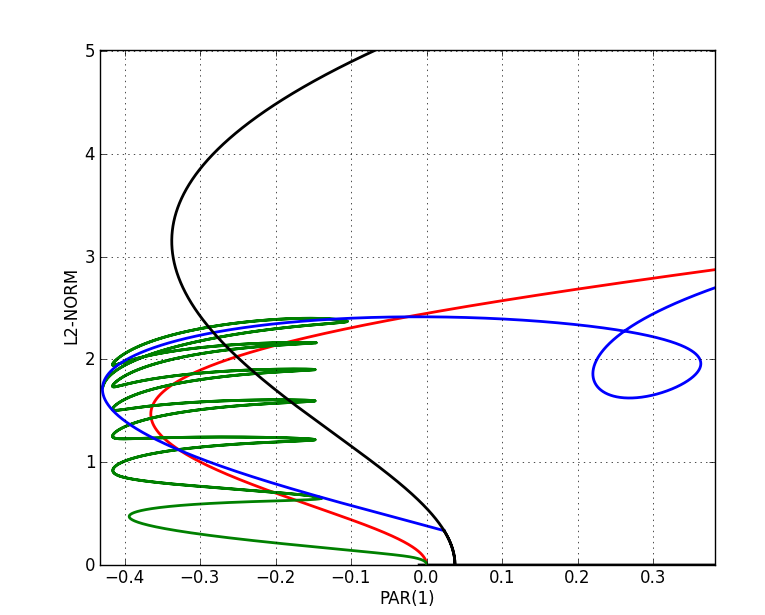
\includegraphics[width=120mm]{BifurcationDiagram1.png}
\caption{\label{fig:bifurcationdiagram1} A Bifurcation diagram for the case that $q=1$ and $\delta=0$, showing a snaking branch that connects two periodic states.}
\end{figure}
}

\newcommand{\FIGdoubleperiod}{
\begin{figure}[htbp]
  \begin{center}
    \mbox{
      \subfloat[solution before the loop]{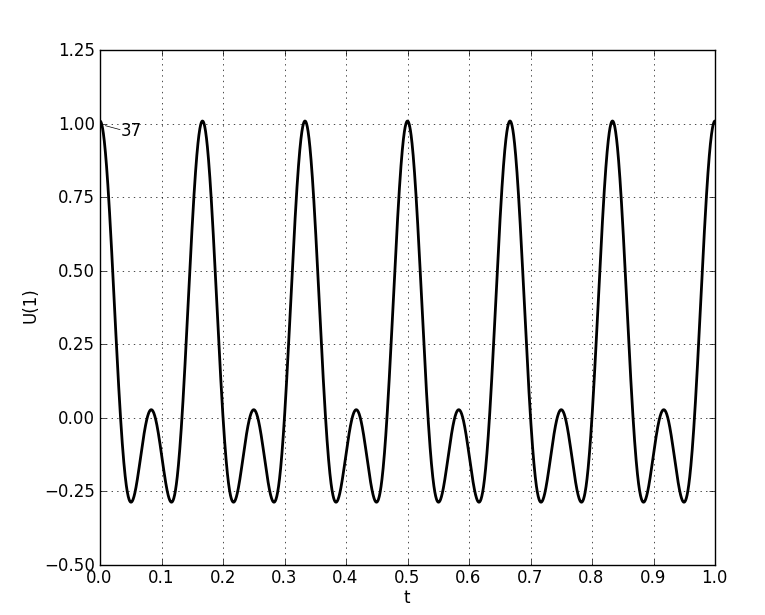
\includegraphics[width=60mm]{dpb24.png}} \quad
      \subfloat[solution after the loop]{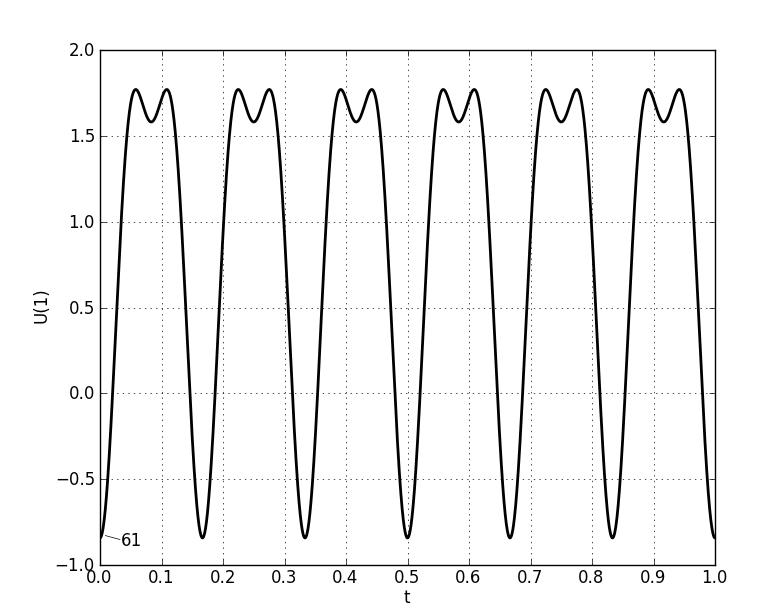
\includegraphics[width=60mm]{dpb24u.png}} 
      }
    \caption{Solutions along periodic branch that bifurcations from $P24$ and connects with the snaking branch from $P20$.}
    \label{fig:doubleperiod1}
  \end{center}
\end{figure}
}

\newcommand{\FIGsnakingA}{
\begin{figure}[htbp]
  \begin{center}
    
      \subfloat[1]{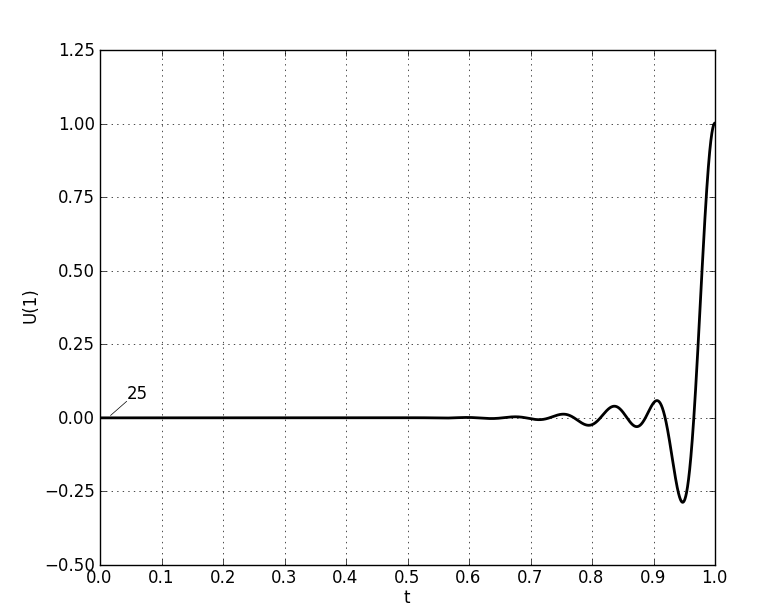
\includegraphics[width=60mm]{sb20a1.png}} \quad
      \subfloat[2]{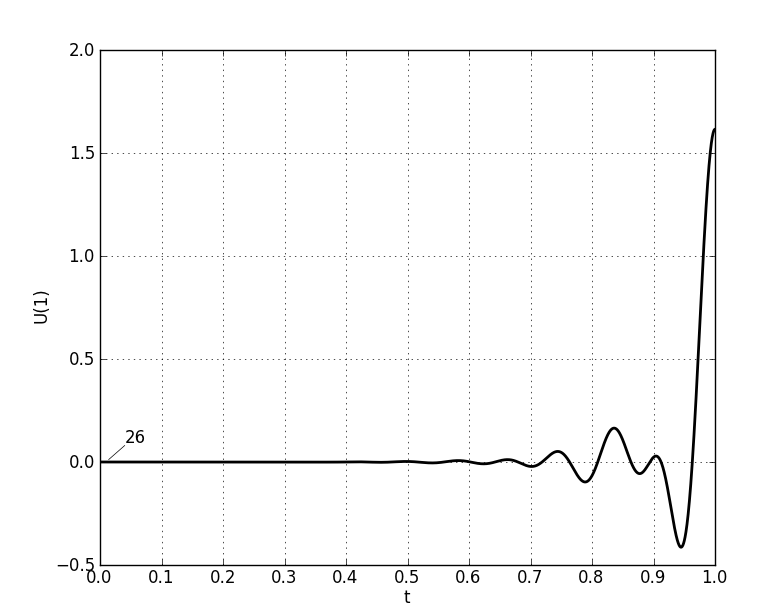
\includegraphics[width=60mm]{sb20a2.png}}\\
      \subfloat[3]{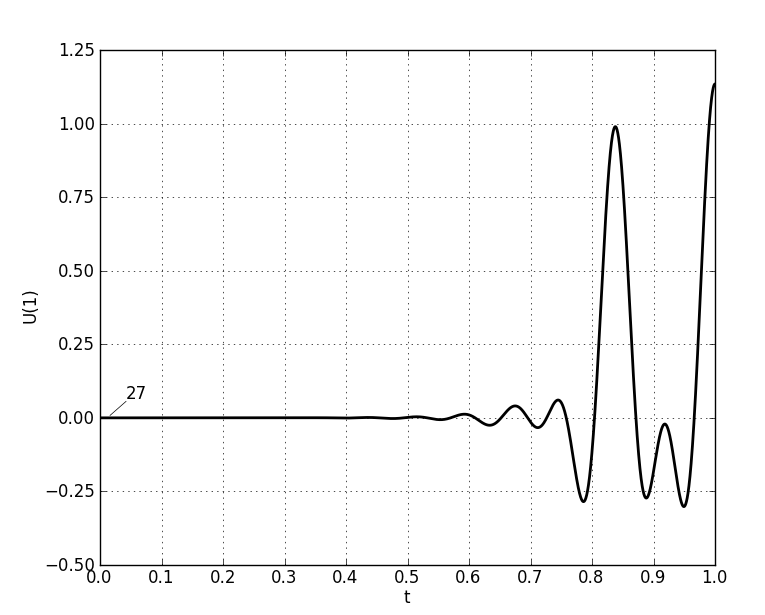
\includegraphics[width=60mm]{sb20a3.png}} \quad
      \subfloat[4]{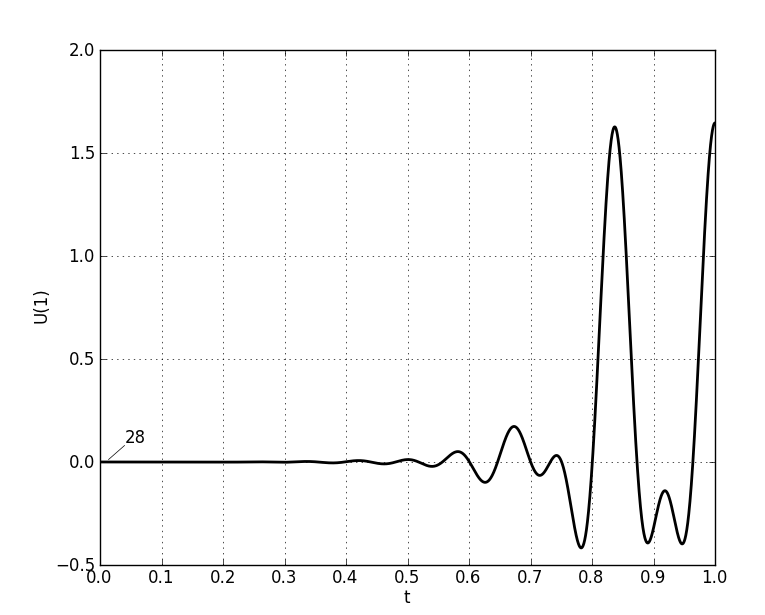
\includegraphics[width=60mm]{sb20a4.png}} 
      
    \caption{Localized solutions along snaking branch that bifurcates from $P20$.}
    \label{fig:snaking1}
  \end{center}
\end{figure}
}


\newcommand{\FIGsnakingmess}{
\begin{figure}[htbp]
  \begin{center}
    \mbox{
      \subfloat[Example solution from third bifurcation point along $P20$]{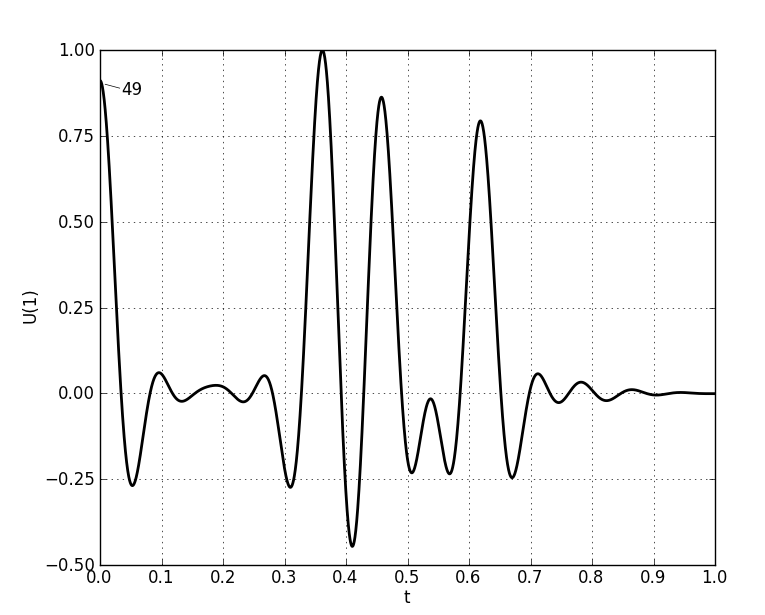
\includegraphics[width=60mm]{sb20cMess.png}} \quad
      \subfloat[Example solution from second bifurcation point along $P24$]{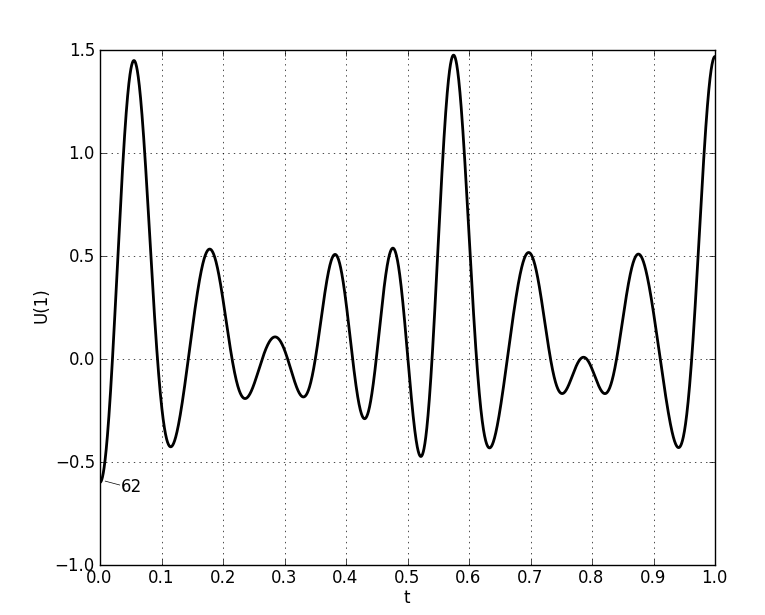
\includegraphics[width=60mm]{sb24bMess.png}} 
      }
    \caption{Examples of solutions with seemingly random pulses. These solutions fall along messy branches that bifurcate from the primary periodic solutions}
    \label{fig:snakingmess1}
  \end{center}
\end{figure}
}


\pagestyle{fancy}
\begin{document}
\preprint{APS/123-QED}

\title{Pattern Formation in a system with competing wavelengths}

\author{Punit Gandhi}
 \email{punit_gandhi@berkeley.edu}
\author{Edgar Knobloch}
 \email{knobloch@berkeley.edu}
\affiliation{Department of Physics, University of California, Berkeley CA 94720, USA}

\begin{abstract}
We propose a modified version of the Swift-Hohenberg equation in an attempt to study a situation in which competition between two patterns of different wavelength exist.
\end{abstract}

\maketitle

\section{Introduction}
The Swift-Hohenberg equation serves as a model for pattern formation in a broad range of physical systems.   This equation, which takes the form  
\begin{equation}
u_t= r u-\left(1+\partial_{x}^2\right)^2u+N[u]\label{eq:SH},
\end{equation}
describes the dynamics of a real field $u$ over one spatial dimension in time, where $N$ is some nonlinear function of $u$.  We have rescaled the equation so that the critical wavenumber that defines the natural wavelength of the patterned state is unity.  We willl be interested in two possible choices of $N$, namely $N_{23}[u]=bu^2-u^3$ and $N_{35}[u]=b u^3-u^5$.  The strength of the linear forcing term $r$ and the strength of the quadratic nonlinearity $b$ are left as parameters of the system.  

There may be physical systems in which multiple patterned states with different characteristic wavelengths can exist simultanously.  We would like to develop a model for such a system and study the interaction and competiton between these patterned states.  We propose a modification to the Swift-Hohenberg equation in which such competition may be possible:
\begin{equation}
u_t= r u-\left(1+\partial_{x}^2\right)^2 \left[\left(q^2+\partial_{x}^2\right)^2+\delta \right] u+N[u]\label{eq:SHm}.
\end{equation}
Linear stability analysis of this equation results in a marginal stability curve (Fig. \ref{fig:marginalstability}) where two wavelengths can compete with each other.  The first wavelength is  $k=1$, just as in the original SHE (Eq. \ref{eq:SH}), and the other occurs at 
\beqn
q_*=\frac{1}{2}\sqrt{1+3q^2 \pm\Delta}.
\eeqn
where $\Delta=\sqrt{(q^2-1)^2-8\delta}$ and $+$/ $-$ is used when $q>1$ and $q<1$ respectively.  We note that such solutions exist only when $(q^2-1)^2>8\delta$, which is the condition that there is a second minimum other than $k=1$ in the marginal stability curve.  The curve that defines the region of interest to us is also proportional to the marginal stability curve of the original Swift-Hohenberg operator with characteristic wavenumber $q$ and forcing $\delta$.  Why is this the case, does it have some physical interpretation?  This is not a constraining restriction since we will generally be interested in small values of $\delta$.
\FIGmarginalstability
When $\delta=0$ and $q_*=q$  both  become unstable at $r=0$. The instability of $q_*$ is shifted for nonzero values of $\delta$ by
\beqn
r_*=\frac{1}{128} \left(3( q^2-1)+\Delta\right)^2 \left( (q^2-1)^2- (q^2-1)\Delta+4 \delta \right).
\eeqn

We will be interested in the case that $\tfrac{8\delta}{(q^2-1)^2}<<1$,  so that the two competing wavelengths will have similar marginal stabilities and can thus compete.  This assumption allows us to approximate $q_*$ and $r_*$ as:
\beqa
q_*&\approx&q\left[1-\frac{4\delta}{(q^2-1)^2}\right] \\
r_*&\approx& (q^2-1)^2 \delta
\eeqa
We note that the $q=1$ is a degenerate case that may need to be handlede seperately.  Another interesting regime could be when $q$ is close to one so that we have nearby wavelengths competing. We might also want to consider the case when $q>>1$ (or $q<<1$) so that the wavelengths of the patterns occur on different lengthscales.  This regime is of interest for quasicrystals?

This equation has been studied by Bentley (2012), though with a slightly different parametrization.  The advantage of this parametrization over the one used by Bentley becomes apparent in the small $\delta$ limit.  We see that $q$ is approximately the wavenumber of the second competing pattern, and $\delta$ is proportional to the relative shift between the onsets of the two patterns.   We might also consider a slightly different parametrization in which the $\delta (1-k^2)^2$ is instead $\delta (1-k^2)$, the so-called "Proctor term" (I think).  The advantage of our parametrization is two-fold: (1) the characteristic wavenumber of one of the patterns is exactly one. (2) The relations between $q_*$, $r_*$ and $q$ and $\delta$ are much simpler in our case.    Bentley has looked at this equation as a model for magnetorotational Taylor-Couette flows.  His focus is in the supercritical regime where the patterned states bifurcate from the homogeneous state with a supercritical pitchforc bifurcation.  He is currently working to publish his work.  We don't know what additional work he has done beyond his thesis that his advisor has shared with us.

Just as in the case of the original Swift-Hohenberg equation (Eq. \ref{eq:SH}), this modified equation can be expressed in terms of a Lyaponuv functional as 
where
\beqn
F[u]=
\eeqn
This implies that the system will always approach a steady state in time, and we can focus on time-independent solutions to give some insight into the dynamics of the system.

\section{Weakly Nonlinear Analysis}
We would like to look at small amplitude solutions in the neighborhood of the $r=0$ bifurcation where the periodic state branches off of the homogeneous state in the space of steady-state solutions.  We will take a multi-scale approach, defining a slow timescale $T=\epsilon^2t$, and long spatial scale $X=\epsilon x$ so that the derivatives become $\partial_t \rightarrow \partial_t+\epsilon^2\partial_T$ and $\partial_x \rightarrow \partial_x+\epsilon\partial_X$.  We will assume that the system will not change on the fast timescale, so we can neglect the $\partial_t$ term. With some trial and error, it can be seen that the appropriate scaling of forcing strength to probe the dynamics we are interested in will be $r=\epsilon^2 \mu$. In addition, we will choose to scale$\delta\rightarrow\epsilon^2 \delta$ so that the difference in onset of instability for the two wavelengths will be of the same order of the forcing that we consider.

The linear part of the modified Swift-Hohenberg equation (Eq.~\ref{eq:SHm}), 
\beqn
L= r-\left(1+\partial_{x}^2\right)^2 \left[\left(q^2+\partial_{x}^2\right)^2+\delta \right],
\eeqn
can be expanded as $L=L_0+\epsilon L_1+\epsilon^2 L_2+...$ where:
\beqa
L_0 &=& -\left(1+\partial_x^2\right)^2 \left(q^2+\partial_x^2\right)^2 \\
L_1 &=& -4\left(1+\partial_x^2\right)  \left(q^2+\partial_x^2\right) \left(1+2 \partial_x^2+q^2\right)\partial_x\partial_X \\
L_2 &=&- 2 \left[14 \partial_x^6+15  \left(q^2+1\right)\partial_x^4+3 \left(q^4+4 q^2+1\right) \partial_x^2+q^2\left(q^2+1\right)\right] \partial_X^2\nonumber\\  
& & -\delta \left[1+ \left(2+\partial_x^2\right)\partial_x^2\right] +\mu -\partial_T \\
L_3 &=& -4   \left[ \left(14 \partial_x^4+10  \left(q^2+1\right)\partial_x^2+q^4+ 4 q^2+1\right)\partial_X^2+\delta\left(1 +\partial_x^2\right)\right]\partial_x \partial_X \\
L_4 &=& -\left[\partial_X^2 \left(70 \partial_x^4+30\left(q^2+1\right) \partial_x^2 +q^4 +4 q^2+1\right)+2 \delta\left(1 +3 \partial_x^2 \right) \right] \partial_X^2  
\eeqa

\subsection{The quadratic-cubic nonlinearity}
We will first consider the case when $N=N_{23}$ so that the modified Swift-Hohenberg equation can be written as $L[u]-N_{23}[u]=0$.  We will assume that the solution can be written as an asymptotic series with the leading term of order $\epsilon$, namely $u=\epsilon u_1 + \epsilon^2 u_2 +\epsilon^2 u_3+...$ 

We can then write out the resulting equation at each order of $\epsilon$ by matching terms at the proper order.
\begin{subequations}
\begin{align}
\mathcal{O}(\epsilon): \:  &-L_0 u_1 =0
\label{eq:msh23o1} \\
\mathcal{O}(\epsilon^2): \: &-L_0 u_2 = L_1 u_1 +b u_1^2
\label{eq:msh23o2} \\
\mathcal{O}(\epsilon^3): \:  &-L_0 u_3 = L_1 u_2 +L_2 u_1 + 2b u_1 u_2-u_1^3
\label{eq:msh23o3}
\end{align}
\end{subequations}
The solution to the $\mathcal{O}(\epsilon)$ equation can be expressed in terms of the yet to be determined complex amplitudes $A_1, B_1$ as:
\beqn
u_1(x,X,T)=A_{11}(X,T)e^{i x} +B_{11}(X,T)e^{i q x} +c.c.
\eeqn
Note that $c.c.$ stands for the complex conjugate of the expression written.  The  $\mathcal{O}(\epsilon^2)$ equation has solutions that can be written inthe form:
\beqa
u_2(x,X,T)&=&C_{20}(X,T) \\
&+ &\left[ A_{21}(X,T)e^{i x}+A_{22}(X,T)e^{2 i x} +B_{21}(X,T)e^{i q x} + B_{22}(X,T)e^{2 i q x} +c.c.\right]
\eeqa
Noting that $L_1 u_1=0$, we see that
\section{Numerical Results}
The steady state solutions of this system as a function of the forcing strength $r$ can be found by numerical continuation.  Auto was used to compute the below bifurcation diagram and solutions.  We have used a domain size of 20 wavelengths for these simulations, but made use of the reflection symmetry to only simulate half.  

\subsection{The one-wavelength case}
The case that $q=1$ and $\delta=0$ is the simplest case to consider since there is only one characteristic wavelength to the problem, namely 1.  We already see a very interesting bifurcation diagram here (Fig. \ref{fig:bifurcationdiagram1}).
\FIGbifurcationdiagramA
The periodic branch bifurcating from the homogeneous solution at $r=0$ has 20 periods and will be called $P20$.  The first secondary bifurcation from $P20$, forms a snaking branch of one-pulse localized states like the ones shown in Fig. \ref{fig:snaking1}.
\FIGsnakingA
This branch eventually reconnects to another periodic branch that does not have a constant amplitude and has 12 periods in the domain (See Fig. \ref{fig:doubleperiod1}.
\FIGdoubleperiod
This periodic solution does not bifurcate from the homogenous solution, but from the $P24$ periodic branch.  It also has a loop in it, where the solution structure inverts so that the small oscillation are on the top instead of the bottom. The bifurcation is  actually the third branch point along the $P24$ branch if followed starting from the homogeneous solution.  The previous two branches along $P24$ are quite messy with seemingly randomly positioned pulses (See Fig. \ref{fig:snakingmess1} for an example).
\FIGsnakingmess  Additionally, we have looked at the solutions formed at the next two bifurcation points along the $P20$ periodic branch.  The second branch snakes with two-pulse localized states while the third branch is messy with seemingly randomly distributed pulses.


\section{Future Work}


\bibliography{WavelengthCompetitonBib}
\end{document}


Realistic systems will not always have a perfectly homogeneous forcing in space, and inhomogeneities may even lead to a way to manipulate dynamics of localized states. As a simple extension to Eq. \ref{eq:SH35}, we would now like to consider the case when the forcing has a periodic perturbation,
\begin{equation}
u_t= r(1+\delta \cos{\kappa x}) u -\left(1+\partial_{x}^2\right)^2u+bu^3-u^5\label{eq:SH35spf}.
\end{equation}

We can make some analytic progress on studying Eq.~\ref{eq:SH35spf} using techniques very similar to those used on the original equation (Eq.~\ref{eq:SH35}). We will look near the $r=0$ bifurcation point on a long timescale and a long spatial scale to get an amplitude equation at leading order.  In the special case that the periodicity of the forcing is half that of the natural wavelength, we obtain a parametrically forced Ginsburg-Landau equation for the amplitude.  

\section{Scaling}
We would like to look at small amplitude solutions in the neighborhood of the $r=0$ bifurcation where the periodic state branches off of the homogeneous state in the space of steady-state solutions.  We will take a multi-scale approach, defining a slow timescale $T=\epsilon^2t$, and long spatial scale $X=\epsilon x$ so that the derivatives become $\partial_t \rightarrow \partial_t+\epsilon^2\partial_T$ and $\partial_x \rightarrow \partial_x+\epsilon\partial_X$.  We will assume that the system will not change on the fast timescale, so we can neglect the $\partial_t$ term. With some trial and error, it can be seen that the appropriate scaling of forcing strength to probe the dynamics we are interested in will be $r=\epsilon^2 \mu$.     Additionally, we will not make any assumptions about $\delta$ yet, but will eventually want to consider the case that $\epsilon <<\delta <<1$.

With this scaling, Eq. \ref{eq:SH35spf} becomes 
\begin{equation}
\epsilon^2 u_T = \epsilon^2 \mu(1+\delta \cos{\kappa x}) u -\left(1+(\partial_{x}+\epsilon \partial_X)^2\right)^2u+bu^3-u^5
\label{eq:SH35spfeps}.
\end{equation}
Note we will also assume that the spatial periodicity of the forcing happens at a lengthscale comparable that of the characteristic wavelength of the patterned state.  In particular, we will focus on the case that $\kappa=2$, as this will lead a parametrically forced Ginzburg-Landau equation.

\section{Expansion}
We will write out the solution as an asymptotic expansion in the small parameter $\epsilon$:
\begin{equation}
u=\sum_{j=0}^{\infty} \epsilon^j u_j
\end{equation}
Since we want to look for small amplitude solutions, we will assume that $u_0=0$ and that the leading order solution comes in only at $\mathcal{O}(\epsilon)$. Furthermore, we can see by the structure of the nonlinear terms that we will not need the even powers of the expansion.  The equation that $u_2$ will need to satisfy, for example, will be identical to the one that $u_1$ will need to satisfy so that we could effectively redefine it by $u_1\rightarrow u_1+\epsilon u_2$.  We will finally note that the leading order effects of the spatially modulated forcing will by captured by making the expansion out to order $\mathcal{O}(\epsilon^3)$.   
\begin{equation}
u=\epsilon u_1 + \epsilon^3 u_3  + \mathcal{O}(\epsilon^5)
\label{eq:AsympExpU}
\end{equation}

We can now plug in the asymptotic series form of the solution Eq. \ref{eq:AsympExpU}) into the scaled version of the SHE35 (Eq. \ref{eq:SH35spfeps}) and match terms in orders of $\epsilon$.  The leading order terms will be $\mathcal{O}(\epsilon)$:
\begin{equation}
u_1+2\partial_x^2 u_1 +\partial_x^4 u_1 = 0.
\end{equation}
This equation has a solution of the form
\begin{equation}
u_1(x,X,T)=A(X,T) e^{i x}+ \bar{A}(X,T) e^{-ix},
\label{eq:u1sol}
\end{equation}
where $A(X,T)$ is a still undetermined complex amplitude that depends only on the slow timescale $T$ and the long lengthscale $X$, and $\bar{A}(X,T)$ is its complex conjugate. Collecting terms at the next order in $\epsilon$ will provide a solvability condition that we will use to determine $A$.

We can now go on to look at the next terms in the expansion, which come in at $\mathcal{O}(\epsilon^3)$:
\begin{eqnarray}
u_3+2\partial_x^2 u_3 &+& \partial_x^4 u_3 =  \nonumber \\
& & -\partial_T u_1-2\partial_X^2 u_1 - 6\partial_x^2 \partial_X^2 u_1 +\mu u_1 +\mu \delta \cos(\kappa x)  u_1 +b u_1^3
\label{eq:AsympExpEps3}
\end{eqnarray}
Plugging in the form of the solution for $u_1$ from Eq. \ref{eq:u1sol} gives the following expression for the RHS of the equation above.
\begin{eqnarray}
\text{RHS}&=&  \nonumber \\ 
& &\left(-A_T  +4 A_{XX}+\mu A + 3b |A|^2 A\right)e^{ix} + \left(-\bar{A}_T +4 \bar{A}_{XX}+\mu \bar{A} + 3b |A|^2 \bar{A}\right)e^{-ix} \nonumber \\
& &+\frac{\mu\delta}{2} A\left(e^{i(1+\kappa)x}+e^{i(1-\kappa)x} \right) + \frac{\mu\delta}{2} \bar{A}\left( e^{-i(1+\kappa)x}+e^{-i(1-\kappa)x} \right) \nonumber \\
& & +bA^3e^{3ix}+b\bar{A}^3e^{-3ix}
\label{eq:RHSeps3}
\end{eqnarray}
The resonant terms of in the above expression (Eq. \ref{eq:RHSeps3}) must vanish in order for this equation to be solved, giving the desired equation that determines the complex amplitude $A$.  The choice of $\kappa$ determines if the effects of the spatially periodic forcing perturbation can be seen at this order.  In particular, the choice of $\kappa=2$, modifies the complex amplitude equation so that it includes a parametric forcing term (proportional to $\bar{A}$).

\section{The 2:1 resonance in the forcing}
We will now focus on the case that the period of the forcing perturbation is half that of the characteristic wavelength of the patterned state, namely that $\kappa=2$.  Plugging this into Eq. \ref{eq:AsympExpEps3} leads to the following equation for the complex amplitude from the solvability condition that resonant terms vanish:
\begin{equation}
-A_T  +4 A_{XX}+\mu A + 3b |A|^2 A+\frac{\mu\delta}{2}\bar{A}=0
\label{eq:LGEpf1}
\end{equation}

With appropriate redefinitions of variables, we can put this equation into the following form
\begin{equation}
A_T  = \mu A + A_{XX} - |A|^2 A+\gamma\bar{A}
\label{eq:LGEpf}
\end{equation}
where we have assumed that $b<0$.

\subsection{Polar Coordinates}
Equation \ref{eq:LGEpf}  can now be put into a form that resembles a particle orbiting in central potential by making the substitution $A=r e^{i\theta}$, where $r$ and $\theta$ are real functions of $X$ and $T$.  The resulting pair of real pde's is:
\begin{subequations}
\begin{align}
\dot{r}&=\mu r - r^3 +r''-r\theta'^2+\gamma r \cos2\theta 
\label{eq:PolarGLEpfr} \\
r^2\dot{\theta}&=2 r r' \theta'+r^2\theta''-\gamma r^2 \sin 2\theta
\label{eq:PolarGLEpfth}
\end{align}
\end{subequations}
where the dot and prime represent derivatives with respect to the time $T$ and the position $X$, respectively.

If we look for steady state solutions in time, we can reduce this problem to an ode with the dependent variable as space instead of time.  We can define a spatial {\it energy} $h$ and {\it angular momentum} $l$ by:
\begin{eqnarray}
l &=& r^2\theta' \\
h &=& \frac{1}{2} r'^2 +\frac{l^2}{2r^2} +\frac{1}{2}\mu r^2 -\frac{1}{4} r^4
\end{eqnarray}
In the limit that $\gamma$ vanishes, these new variables are actually constants of motion of the amplitude Eq. \ref{eq:LGEpf}.  The problem described by Eq. \eqref{eq:PolarGLEpfr} and \eqref{eq:PolarGLEpfth} can be mapped onto the problem of a particle traveling in a central potential equivilent to a particle in a central potential if we consider dynamics in space instead of time.  The spatial energy $h$ has a kinetic term, a effective potential term from the spatial angular momentum $l$, and a central potental well term.  Equations \eqref{eq:PolarGLEpfr} and \eqref{eq:PolarGLEpfth} can now be rewritten in terms of the spatial energy and angular momentum as:
\begin{subequations}
\begin{align}
l' &= \gamma r^2 \sin 2\theta 
\label{eq:CentPotL} \\
h'&= \gamma l \sin 2\theta-\gamma r r' \cos 2\theta
\label{eq:CentPotH}
\end{align}
\end{subequations}

Assuming $\epsilon <<\gamma <<1$ allows us to treat $l$ and $h$ as slowly varying quantities.  We could, in principle, apply the method of averaging to this equation to get spatially averaged equations that depend only on $l$ and $h$.  We would assume that these two quantities are constant and integrate over one period to average out the small variations of $r$ and $\theta$.  Unfortunately, this involves integrals that I'm not exactly sure how to do.

We can use the interpretation of a particle in a central potential to help us find solutions to our original problem that are localized in space and steady-state in time.  These type of solutions correspond to  orbits of the particle that approach $r=0$ as $x\rightarrow \pm \infty$.  We could look for these kinds of solutions to the unperturbed problem (when $\gamma=0$) and then try to understand what the perturbation does to these solutions. 

We can further simplify the energy equation by noting that the RHS is the spatial derivative of the quantity $-\half \gamma r^2 \cos 2 \theta$. By redefining the energy as
\beqn
\bar{h}=\frac{1}{2} r'^2 +\frac{l^2}{2r^2} +\frac{1}{2}\mu r^2 -\frac{1}{4} r^4+\half \gamma r^2 \cos 2 \theta,
\label{eq:CowboyHat}
\eeqn
so that the potential is no longer radially symmetric.  A plot of this potential, which will be referred to as the {\it cowboy hat potential}, is shown in Fig. \ref{fig:CowboyHat}.
\FIGcowboy
The force corresponding the additional energy term is $\mathbf{F}=\gamma r (\cos2\theta \;\hat{r} - \sin2\theta \; \hat{\theta})$ is plotted in Fig. \ref{fig:CowboyForce}. 
\FIGforce

\bibliography{SpatialForcingBib}
\end{document}




